    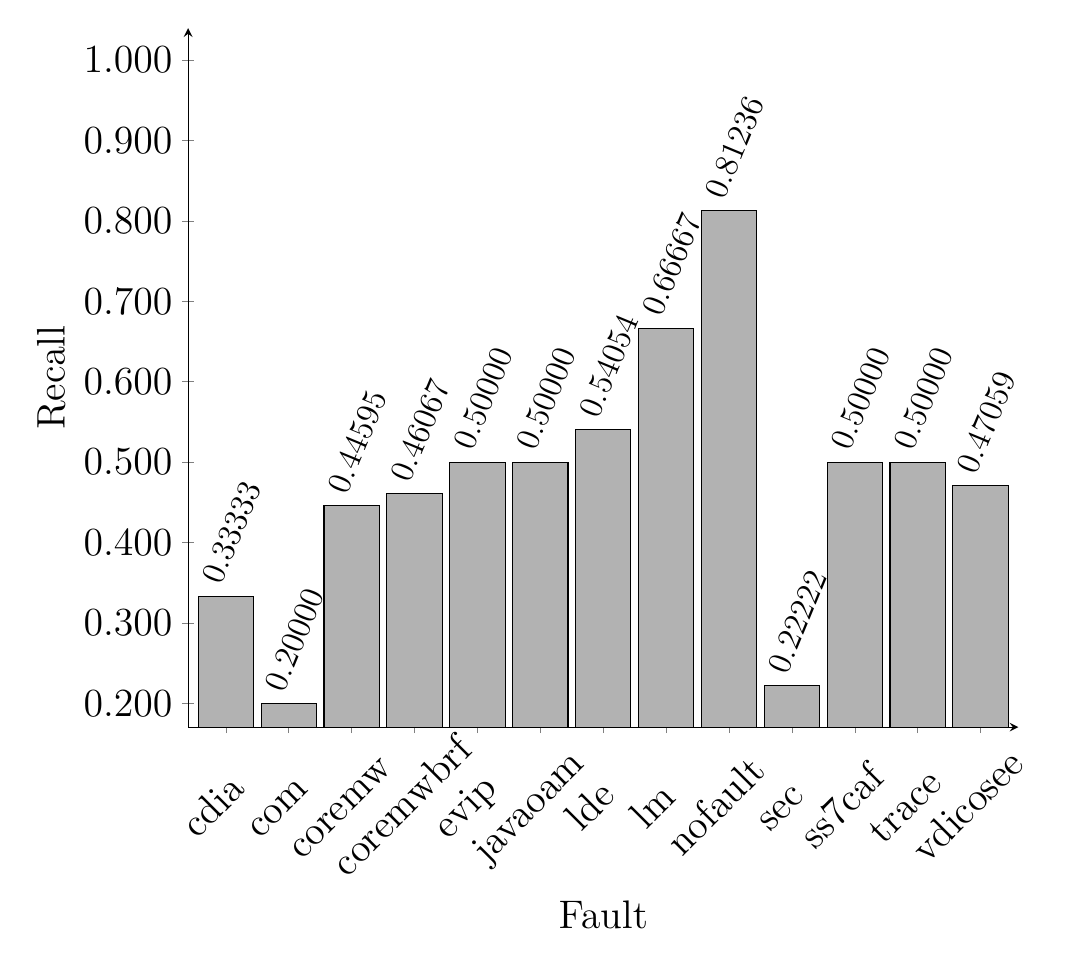
\begin{tikzpicture}[font=\Large]
    \begin{axis}[
      width=\textwidth,
      ybar,
      font=\Large,
      bar width=20pt,
      xlabel={Fault},
      ylabel={Recall},
      xticklabel style={rotate=45,anchor=base,yshift=-20,xshift=-22},
      xtick=data,
      ymin=0.2100,
      ymax=1.00,
      axis x line=bottom,
      axis y line=left,
      enlarge x limits=0.1,
      enlargelimits=0.05,
      domain=0.21:1.000,
              y tick label style={
            /pgf/number format/.cd,
            fixed,
            zerofill,
            precision=3,
            /tikz/.cd,},
      symbolic x coords={cdia,com,coremw,coremwbrf,evip,javaoam,lde,lm,nofault,sec,ss7caf,trace,vdicosee},
      nodes near coords={\pgfmathprintnumber[fixed zerofill, precision=5]{\pgfplotspointmeta}},
      every node near coord/.append style={color=black, rotate=67.5, anchor=center, font=\large, xshift=22, yshift=7}],

    ]
      \addplot[fill=black!30] coordinates {
        (cdia,0.33333) (com,0.2) 
		(coremw,.445946) (coremwbrf,0.460674) (evip,0.5) (javaoam, 0.5) (lde, 0.540541) (lm, 0.666667) (nofault,0.812364) (sec, 0.222222) (ss7caf, .5) (trace, 0.5) (vdicosee,0.470588)
      };
    \end{axis}
  \end{tikzpicture}